%% BioMed_Central_Tex_Template_v1.06
%%                                      %
%  bmc_article.tex            ver: 1.06 %
%                                       %

%%IMPORTANT: do not delete the first line of this template
%%It must be present to enable the BMC Submission system to
%%recognise this template!!

%%%%%%%%%%%%%%%%%%%%%%%%%%%%%%%%%%%%%%%%%
%%                                     %%
%%  LaTeX template for BioMed Central  %%
%%     journal article submissions     %%
%%                                     %%
%%          <8 June 2012>              %%
%%                                     %%
%%                                     %%
%%%%%%%%%%%%%%%%%%%%%%%%%%%%%%%%%%%%%%%%%


%%%%%%%%%%%%%%%%%%%%%%%%%%%%%%%%%%%%%%%%%%%%%%%%%%%%%%%%%%%%%%%%%%%%%
%%                                                                 %%
%% For instructions on how to fill out this Tex template           %%
%% document please refer to Readme.html and the instructions for   %%
%% authors page on the biomed central website                      %%
%% http://www.biomedcentral.com/info/authors/                      %%
%%                                                                 %%
%% Please do not use \input{...} to include other tex files.       %%
%% Submit your LaTeX manuscript as one .tex document.              %%
%%                                                                 %%
%% All additional figures and files should be attached             %%
%% separately and not embedded in the \TeX\ document itself.       %%
%%                                                                 %%
%% BioMed Central currently use the MikTex distribution of         %%
%% TeX for Windows) of TeX and LaTeX.  This is available from      %%
%% http://www.miktex.org                                           %%
%%                                                                 %%
%%%%%%%%%%%%%%%%%%%%%%%%%%%%%%%%%%%%%%%%%%%%%%%%%%%%%%%%%%%%%%%%%%%%%

%%% additional documentclass options:
%  [doublespacing]
%  [linenumbers]   - put the line numbers on margins

%%% loading packages, author definitions

%\documentclass[twocolumn]{bmcart}% uncomment this for twocolumn layout and comment line below
\documentclass{bmcart}

%%% Load packages
%\usepackage{amsthm,amsmath}
%\RequirePackage{natbib}
%\RequirePackage[authoryear]{natbib}% uncomment this for author-year bibliography
%\RequirePackage{hyperref}
\usepackage[utf8]{inputenc} %unicode support
\usepackage{apacite}
\usepackage{appendix}
\usepackage{amsmath}
\usepackage{amsthm}
% for ASY interactive 3d figure
%\usepackage[inline]{asymptote}
\usepackage{amssymb} % for approx greater than
%\usepackage{caption}
\usepackage{placeins} % for \FloatBarrier
\usepackage{graphicx}
\usepackage{subcaption}
\usepackage{longtable}
\usepackage{setspace}
\usepackage{booktabs}
\usepackage{tabularx}
\usepackage{xcolor,colortbl}
\usepackage{chngpage}
\usepackage{natbib}
%\bibpunct{(}{)}{,}{a}{}{;} 
\usepackage{url}
\usepackage{nth}
\usepackage{authblk}
\usepackage[most]{tcolorbox}
\usepackage[normalem]{ulem}
\usepackage{amsfonts}
\usepackage{censor}
\usepackage{etoolbox}
\AtBeginEnvironment{quote}{\singlespace\small}
\AtEndEnvironment{quote}{\endsinglespace}
%\usepackage[applemac]{inputenc} %applemac support if unicode package fails
%\usepackage[latin1]{inputenc} %UNIX support if unicode package fails


%%%%%%%%%%%%%%%%%%%%%%%%%%%%%%%%%%%%%%%%%%%%%%%%%
%%                                             %%
%%  If you wish to display your graphics for   %%
%%  your own use using includegraphic or       %%
%%  includegraphics, then comment out the      %%
%%  following two lines of code.               %%
%%  NB: These line *must* be included when     %%
%%  submitting to BMC.                         %%
%%  All figure files must be submitted as      %%
%%  separate graphics through the BMC          %%
%%  submission process, not included in the    %%
%%  submitted article.                         %%
%%                                             %%
%%%%%%%%%%%%%%%%%%%%%%%%%%%%%%%%%%%%%%%%%%%%%%%%%


% Toggle show graphics
%\def\includegraphic{}
%\def\includegraphics{}



%%% Put your definitions there:
\startlocaldefs
\endlocaldefs


%%% Begin ...
\begin{document}

%%% Start of article front matter
\begin{frontmatter}

\begin{fmbox}
\dochead{Research}

%%%%%%%%%%%%%%%%%%%%%%%%%%%%%%%%%%%%%%%%%%%%%%
%%                                          %%
%% Enter the title of your article here     %%
%%                                          %%
%%%%%%%%%%%%%%%%%%%%%%%%%%%%%%%%%%%%%%%%%%%%%%

\title{Independent time measures}

%%%%%%%%%%%%%%%%%%%%%%%%%%%%%%%%%%%%%%%%%%%%%%
%%                                          %%
%% Enter the authors here                   %%
%%                                          %%
%% Specify information, if available,       %%
%% in the form:                             %%
%%   <key>={<id1>,<id2>}                    %%
%%   <key>=                                 %%
%% Comment or delete the keys which are     %%
%% not used. Repeat \author command as much %%
%% as required.                             %%
%%                                          %%
%%%%%%%%%%%%%%%%%%%%%%%%%%%%%%%%%%%%%%%%%%%%%%

\author[
   addressref={aff1},                   % id's of addresses, e.g. {aff1,aff2}
   corref={aff1},                       % id of corresponding address, if any
   noteref={n1},                        % id's of article notes, if any
   email={riffe@demogr.mpg.de}   % email address
]{\inits{TR}\fnm{Tim} \snm{Riffe}}
\author[
   addressref={aff2, aff3},
   email={cohen@mail.rockefeller.edu}
]{\inits{JEC}\fnm{Joel E.} \snm{Cohen}}

%%%%%%%%%%%%%%%%%%%%%%%%%%%%%%%%%%%%%%%%%%%%%%
%%                                          %%
%% Enter the authors' addresses here        %%
%%                                          %%
%% Repeat \address commands as much as      %%
%% required.                                %%
%%                                          %%
%%%%%%%%%%%%%%%%%%%%%%%%%%%%%%%%%%%%%%%%%%%%%%

\address[id=aff1]{%                           % unique id
  \orgname{Max-Planck-Institute for Demographic Research} % university, etc
 % \street{Konrad-Zuse-Str 1},                     %
 % \postcode{18057}                                % post or zip code
 % \city{Rostock},                              % city
 % \cny{DE}                                    % country
}
\address[id=aff2]{%
  \orgname{The Rockefeller University}
 % \street{D\"{u}sternbrooker Weg 20},
 % \postcode{24105}
 % \city{Kiel},
 % \cny{Germany}
}
\address[id=aff3]{%
  \orgname{Columbia University}
  %\street{D\"{u}sternbrooker Weg 20},
  %\postcode{24105}
  %\city{Kiel},
  %\cny{Germany}
}

%%%%%%%%%%%%%%%%%%%%%%%%%%%%%%%%%%%%%%%%%%%%%%
%%                                          %%
%% Enter short notes here                   %%
%%                                          %%
%% Short notes will be after addresses      %%
%% on first page.                           %%
%%                                          %%
%%%%%%%%%%%%%%%%%%%%%%%%%%%%%%%%%%%%%%%%%%%%%%

\begin{artnotes}
%\note{Sample of title note}     % note to the article
\note[id=n1]{Equal contributor} % note, connected to author
\end{artnotes}

\end{fmbox}% comment this for two column layout

%%%%%%%%%%%%%%%%%%%%%%%%%%%%%%%%%%%%%%%%%%%%%%
%%                                          %%
%% The Abstract begins here                 %%
%%                                          %%
%% Please refer to the Instructions for     %%
%% authors on http://www.biomedcentral.com  %%
%% and include the section headings         %%
%% accordingly for your article type.       %%
%%                                          %%
%%%%%%%%%%%%%%%%%%%%%%%%%%%%%%%%%%%%%%%%%%%%%%

\begin{abstractbox}

\begin{abstract} % abstract
\parttitle{Background} 
The demographic time identity consists in a linear relationship between all pairs of six fundamental time measures: age, period, cohort, time to death, length of life, and time of death. Certain subsets of time measures in this and other higher order identities consist in time measures that are independent of one another.
\parttitle{Objective} 
We aim to describe the relationship between
independent time measures and the identities within which they are nested, with special attention to the demographic time identity and its three independent time dyads. We also aim to determine whether data structured on such time dyads might be useful in demographic research.
\parttitle{Data and Methods} 
We illustrate concepts visually based on data from the Colonial Qu\'{e}bec Population Register and from the US Health and Retirement study.
\parttitle{Results} 
We show that a Cartesian mapping of independent time dyads form a redundant mapping of the same demographic timespace. These add three previously undescribed demographic perspectives to the four Lexis-like perspectives, for a total of seven proposed standard perspectives. 
\parttitle{Conclusions} 
We show independent sets of time measures to be consistent with the temporal identities within which they are nested. We demonstrate that these perspectives can be useful for pattern detection and characterization in demographic research.
\end{abstract}

%%%%%%%%%%%%%%%%%%%%%%%%%%%%%%%%%%%%%%%%%%%%%%
%%                                          %%
%% The keywords begin here                  %%
%%                                          %%
%% Put each keyword in separate \kwd{}.     %%
%%                                          %%
%%%%%%%%%%%%%%%%%%%%%%%%%%%%%%%%%%%%%%%%%%%%%%

\begin{keyword}
\kwd{sample}
\kwd{article}
\kwd{author}
\end{keyword}

% MSC classifications codes, if any
%\begin{keyword}[class=AMS]
%\kwd[Primary ]{}
%\kwd{}
%\kwd[; secondary ]{}
%\end{keyword}

\end{abstractbox}
%
%\end{fmbox}% uncomment this for twcolumn layout

\end{frontmatter}

%%%%%%%%%%%%%%%%%%%%%%%%%%%%%%%%%%%%%%%%%%%%%%
%%                                          %%
%% The Main Body begins here                %%
%%                                          %%
%% Please refer to the instructions for     %%
%% authors on:                              %%
%% http://www.biomedcentral.com/info/authors%%
%% and include the section headings         %%
%% accordingly for your article type.       %%
%%                                          %%
%% See the Results and Discussion section   %%
%% for details on how to create sub-sections%%
%%                                          %%
%% use \cite{...} to cite references        %%
%%  \cite{koon} and                         %%
%%  \cite{oreg,khar,zvai,xjon,schn,pond}    %%
%%  \nocite{smith,marg,hunn,advi,koha,mouse}%%
%%                                          %%
%%%%%%%%%%%%%%%%%%%%%%%%%%%%%%%%%%%%%%%%%%%%%%

%%%%%%%%%%%%%%%%%%%%%%%%% start of article main body
% <put your article body there>

\section*{Background}

Dated events on a timeline form the foundation of numerous empirical approaches to detect, estimate, and describe patterns in processes and outcomes in the social sciences. Process patterns might be called transitions, and there are several varieties of these (continuous/discrete, conditional/unconditional, forward/backward \citep{brouard2019backward}, and more). Outcome patterns refer to either things such as prevalence, distribution properties (e.g. expectancies), sequences, episode statistics, and others. Outcome patterns can either be calculated from a process model or observed directly from data. Examples of process patterns include age-structured rates of fertility, mortality, and migration. Examples of outcome patterns include trends in length of life, healthy life expectancy, counts of births structured in some way, or employment trajectories. 

This paper deals with the calendar relationships that underpin all such knowledge of the world. Most empirical work that describes processes and outcomes makes use of a limited subset of the temporal structure that is available, and often the implications of relationships between time measures are unrecognized. Previous work \citep{riffe2017demographictime} formalizes the relationship between events in time, and the durations between them. A given set of event types determines a further set of durations. Taken together, a set of events and their implied durations comprise a dense linear relationship that one might call a temporal \emph{identity}. The most common of these in empirical demographic research is the \emph{Lexis} identity between period (date), cohort(date), and age (duration). There are countless Lexis-like relationships between linearly dependent time measures, and these can be combined into higher-order Lexis identities. 

A primary example of a higher order Lexis identity is the so-called \emph{demographic time identity}, which defines a relationship between age (A), period (P), cohort (C), time until death (T), time of death (D), and length of life (L). In describing the demographic time identity, \citet{riffe2017demographictime} give an almost exhaustive account of the so-called \emph{informative} and \emph{uninformative} dyads. Informative dyads are those sets of two time measures (from APCTDL) that imply a third time measure via identity. For example, AP implies C. Four such 3-part (triad) identities are described at length, with examples and diagram depiction (APC, TPD, CPD, TAL). Uninformative dyads are sets of two time measures that do not directly relate, and which therefore do not imply a third time measure. The three examples given are LP, AD, and CT, which are depicted in the authors' Tab.~(2) and discussed in the text as follows:
\begin{quote}
Triad identities are more meaningful than uninformative dyads. This is so even in the absence of data, due to the underlying relationship between measures. Each of the triad identities can accommodate some version of a lifeline, for instance \citep[p5][]{riffe2017demographictime}. 
\end{quote}

Contrary to the above, in the present note we aim to show how uninformative dyads can reveal meaningful relationships in data. For better semantics and precision, we suggest calling these \emph{independent} dyads rather than uninformative dyads. We relate independent dyad diagrams to lifelines in two dimensions (2d). We relate 2d independent planes to the three-dimensional (3d) demographic time identity, showing how these are also cross-sections of the same 3d volume, but which follow a cubic rather than a tetrahedral structure. We show how data structured on independent time measures may still reveal meaningful patterns using historical data from Qu\'{e}bec. We speculate on a way to view and interpret data structured by the demographic time identity using arbitrarily defined planes as cross-sections. We speculate on how data structured by independent time measures may be meaningful in general.

\section*{Geometric relationships}
  The demographic time identity can be represented as a tetrahedral graph, with time measures mapped to the six edges of a tetrahedron. The four Lexis-like identities are found on the faces of the tetrahedron. The identity fills a 3d space because tetrahedra tessellate with octahedra in a 2:1 ratio. \citet{riffe2017demographictime} considered neither independent pairs of time measures nor the significance of octahedra in this geometric construct. Figure~\ref{fig:tet} shows the tetrahedral graph of the demographic time identity among age (A), period (P), cohort (C), time to death (T), death cohort (D), and length of life (L). Independent dyads are those that do not share any vertex in the graph, and these appear as disjoint and perpendicular in the present 2d graph representation, though they are not perpendicular in 3d space: CT, LP, and AD.

\begin{figure}[h!]
\centering
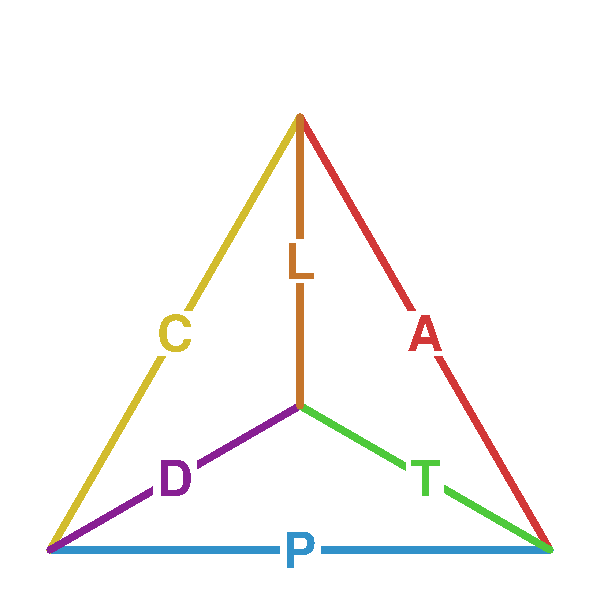
\includegraphics[width=4in]{Figures/TetraHedronEdgesOnly.pdf}
\caption{Tetrahedral graph of demographic time hexad identity, with edges
labelled by the six time indices. Reproduced from 
\citet{riffe2017demographictime}.}
\label{fig:tet}
\end{figure}

 In a triad identity there are no independent dyads, but in the demographic time identity there are three independent dyads, each consisting in an event paired with a duration defined as the interval between the other two dated events. In general, a time identity defined on the basis of $n$ events implies a graph with $n+1$ vertices, implying a total of $\binom{n+1}{2}$ graph edges. Each edge in the graph represents a time measure. Since $n$ of the edges are calendar-event measures, $\binom{n+1}{2} - n$ are duration measures. The $n$ calendar-dated measures are represented as graph edges sharing a single vertex. Triad identities are found wherever two edges share a vertex, for a total of three vertices, which means there must be $\binom{n+1}{3}$ of them within an identity. Independent dyads are pairs of edges that do not share a vertex, meaning that they use four vertices. Since there are $\binom{n+1}{2}$ ways to select one edge, there are $\binom{n-1}{2}$ ways to do so after having removed the two vertices of the first edge, or $\frac{1}{2}\binom{n+1}{2}\binom{n-1}{2}$ unique ways to select two unconnected edges, which simplifies to $3\binom{n+1}{4}$ independent dyads. For a more complicated example, a multistate model of period, birth, marriage, divorce, and death ($n=5$) would therefore imply 45 independent dyads, and a total of 20 triad identities. As $n$ increases, the fraction of possible temporal dyads that are independent approaches 1. To illustrate this point think of the universe of all dates and the potential durations between them: Pick two out of this massive urn and they will almost certainly be independent in this sense.

Any pair of quantitative variables can define the axes of a standard Cartesian plane. When Cartesian axes are defined by two independent time measures and in equal time units, the resultant plane is an isometric projection. Let's call this an independent plane for short. There are two ways that an independent plane may be treated: either (i) accounting for a larger temporal identity or (ii) not. Here we limit comments to the 3d case of the demographic time identity. For the first kind (i) planes are cross-sections of the same 3d demographic timespace previously defined in Fig.~\ref{fig:tet}, and the independent dyads can also be conceived of as \emph{axes of view} on the demographic timespace. This idea is described further in Sec.~\ref{sec:viewaxes}. For the second kind (ii), independent planes are the same as any standard Cartesian plane used in data analyses: patterns revealed could be due to real structure or due to sample heterogeneity in other time measures. That is, the larger temporal identity within which these independent measures are nested is \emph{flattened}.

\subsection*{View axes}
\label{sec:viewaxes}
Imagine now the 3d projection of the graph from Fig.~\ref{fig:tet}, a regular tetrahedron. An angle of view directly at any of the four faces of the demographic time tetrahedron reveals the plane-perspective of a Lexis-like identity. In other words, the viewing axis is set as \emph{normal} to one of the faces of the tetrahedron. Interactive Fig.~\ref{fig:viewaxes} may help visualize the notion of viewing axes--- the view on a plane is orthogonal if an axis line is reduced to appear as a point in the centroid of the tetrahedron. The view axes of the four triad identities map to the four medians (axes of 3-fold symmetry) of the tetrahedron, depicted in Fig.~\ref{fig:depviewaxes} with cyan colored lines. Independent dyad planes are revealed when the viewing angle is such that the midpoints of opposite tetrahedral edges are aligned. There are three pairs of opposite edges (LP, TC, AD), and therefore three viewing angles of this kind, which map to the bimedians of the tetrahedron (axes of 2-fold symmetry), depicted in Figure~\ref{fig:indepviewaxes} with magenta lines.

\begin{figure}
\begin{subfigure}[t]{0.45\linewidth}
    \centering
    %\begin{asy}
// DepViewAxes produced by rgl
settings.prc = true;
size(3inches, 3inches);
import graph3;
currentprojection = orthographic(0, -3.101144, 1.128724, up = (0, 0.3420201, 0.9396926));
defaultpen(fontsize(14));
ticklabel RGLstrings(real[] at, string[] label)
{
  return new string(real x) {
    int i = search(at, x);
    if (i < 0) return "";
    else return label[i];
  };
}

ticklabel RGLScale(real s)
{
  return new string(real x) {return format(s*x);};
}
currentlight = light(ambient=new pen[] {rgb(1,1,1)},
diffuse = new pen[] {rgb(1,1,1)},
specular = new pen[] {rgb(1,1,1)},
position = new triple[] {(0,0,1)},
viewport = true);
currentpen += linewidth(4);
currentpen = colorless(currentpen) + rgb(0.1921569, 0.5686275, 0.7882353);
draw((0.4985029, 0, -0.1762474)
--(-0.2492514, 0.4317162, -0.1762474)
);
label("P", position = (-0.002741766, 0.3181748, -0.1938721), align = (0,0));
currentpen = colorless(currentpen) + rgb(0.8235294, 0.7372549, 0.1764706);
draw((0.4985029, 0, -0.1762474)
--(-0.2492514, -0.4317162, -0.1762474)
);
label("C", position = (-0.002741766, -0.3181748, -0.1938721), align = (0,0));
currentpen = colorless(currentpen) + rgb(0.5333334, 0.1215686, 0.5764706);
draw((0.4985029, 0, -0.1762474)
--(0, 0, 0.5287422)
);
label("D", position = (0.1809565, 0, 0.3257052), align = (0,0));
currentpen = colorless(currentpen) + rgb(0.8235294, 0.2156863, 0.2156863);
draw((-0.2492514, 0.4317162, -0.1762474)
--(-0.2492514, -0.4317162, -0.1762474)
);
label("A", position = (-0.2741766, -0.1614619, -0.1938721), align = (0,0));
currentpen = colorless(currentpen) + rgb(0.3058824, 0.7882353, 0.2313726);
draw((-0.2492514, 0.4317162, -0.1762474)
--(0, 0, 0.5287422)
);
label("T", position = (-0.09047827, 0.156713, 0.3257052), align = (0,0));
currentpen = colorless(currentpen) + rgb(0.772549, 0.4588235, 0.1686275);
draw((-0.2492514, -0.4317162, -0.1762474)
--(0, 0, 0.5287422)
);
label("L", position = (-0.09047827, -0.156713, 0.3257052), align = (0,0));
currentpen += linewidth(2);
currentpen = colorless(currentpen) + rgb(0, 1, 1);
draw((0, 0, 0.6873648)
--(0, 0, -0.2291216)
);
currentpen = colorless(currentpen) + rgb(0, 0, 0);
label("APC", position = (0, 0, -0.2291216), align = (0,0));
currentpen = colorless(currentpen) + rgb(0, 1, 1);
draw((-0.3240269, -0.561231, -0.2291216)
--(0.108009, 0.187077, 0.07637387)
);
currentpen = colorless(currentpen) + rgb(0, 0, 0);
label("TPD", position = (0.108009, 0.187077, 0.07637387), align = (0,0));
currentpen = colorless(currentpen) + rgb(0, 1, 1);
draw((-0.3240269, 0.561231, -0.2291216)
--(0.108009, -0.187077, 0.07637387)
);
currentpen = colorless(currentpen) + rgb(0, 0, 0);
label("CDL", position = (0.108009, -0.187077, 0.07637387), align = (0,0));
currentpen = colorless(currentpen) + rgb(0, 1, 1);
draw((0.6480538, 0, -0.2291216)
--(-0.2160179, 0, 0.07637387)
);
currentpen = colorless(currentpen) + rgb(0, 0, 0);
label("TAL", position = (-0.2160179, 0, 0.07637387), align = (0,0));
currentlight.background = rgb(0.2980392, 0.2980392, 0.2980392);
currentlight.background = rgb(1, 1, 1);
currentlight.background = rgb(1, 1, 1);
\end{asy}

    \caption{The four view axes of the triad dependencies map to the medians of the tetrahedron. Rotate the tetrahedron so that a given cyan line is reduced to a point: The resulting view is then orthogonal to the outermost identity when flattened to 2d.}
    \label{fig:depviewaxes}
\end{subfigure}
~~
\begin{subfigure}[t]{0.45\linewidth}
    %\begin{asy}
// IndepViewAxes produced by rgl
settings.prc = true;
size(3inches, 3inches);
import graph3;
currentprojection = orthographic(0, -2.640817, 0.9611788, up = (0, 0.3420201, 0.9396926));
defaultpen(fontsize(14));
ticklabel RGLstrings(real[] at, string[] label)
{
  return new string(real x) {
    int i = search(at, x);
    if (i < 0) return "";
    else return label[i];
  };
}

ticklabel RGLScale(real s)
{
  return new string(real x) {return format(s*x);};
}
currentlight = light(ambient=new pen[] {rgb(1,1,1)},
diffuse = new pen[] {rgb(1,1,1)},
specular = new pen[] {rgb(1,1,1)},
position = new triple[] {(0,0,1)},
viewport = true);
currentpen += linewidth(4);
currentpen = colorless(currentpen) + rgb(0.1921569, 0.5686275, 0.7882353);
draw((0.5820827, 0, -0.2057973)
--(-0.2910413, 0.5040984, -0.2057973)
);
label("P", position = (-0.003201455, 0.3715205, -0.226377), align = (0,0));
currentpen = colorless(currentpen) + rgb(0.8235294, 0.7372549, 0.1764706);
draw((0.5820827, 0, -0.2057973)
--(-0.2910413, -0.5040984, -0.2057973)
);
label("C", position = (-0.003201455, -0.3715205, -0.226377), align = (0,0));
currentpen = colorless(currentpen) + rgb(0.5333334, 0.1215686, 0.5764706);
draw((0.5820827, 0, -0.2057973)
--(0, 0, 0.6173919)
);
label("D", position = (0.211296, 0, 0.3803134), align = (0,0));
currentpen = colorless(currentpen) + rgb(0.8235294, 0.2156863, 0.2156863);
draw((-0.2910413, 0.5040984, -0.2057973)
--(-0.2910413, -0.5040984, -0.2057973)
);
label("A", position = (-0.3201455, -0.1885328, -0.226377), align = (0,0));
currentpen = colorless(currentpen) + rgb(0.3058824, 0.7882353, 0.2313726);
draw((-0.2910413, 0.5040984, -0.2057973)
--(0, 0, 0.6173919)
);
label("T", position = (-0.105648, 0.1829877, 0.3803134), align = (0,0));
currentpen = colorless(currentpen) + rgb(0.772549, 0.4588235, 0.1686275);
draw((-0.2910413, -0.5040984, -0.2057973)
--(0, 0, 0.6173919)
);
label("L", position = (-0.105648, -0.1829877, 0.3803134), align = (0,0));
currentpen += linewidth(2);
currentpen = colorless(currentpen) + rgb(1, 0, 1);
draw((-0.436562, 0, -0.308696)
--(0.436562, 0, 0.308696)
);
currentpen = colorless(currentpen) + rgb(0, 0, 0);
label("AD", position = (-0.4656661, 0, -0.3292757), align = (0,0));
currentpen = colorless(currentpen) + rgb(1, 0, 1);
draw((-0.218281, 0.3780738, 0.308696)
--(0.218281, -0.3780738, -0.308696)
);
currentpen = colorless(currentpen) + rgb(0, 0, 0);
label("TC", position = (-0.2328331, 0.4032787, 0.3292757), align = (0,0));
currentpen = colorless(currentpen) + rgb(1, 0, 1);
draw((-0.218281, -0.3780738, 0.308696)
--(0.218281, 0.3780738, -0.308696)
);
currentpen = colorless(currentpen) + rgb(0, 0, 0);
label("LP", position = (-0.2328331, -0.4032787, 0.3292757), align = (0,0));
currentlight.background = rgb(0.2980392, 0.2980392, 0.2980392);
currentlight.background = rgb(1, 1, 1);
currentlight.background = rgb(1, 1, 1);
\end{asy}

    \caption{The three view axes of the independent planes map to the bimedians of the tetrahedron. Rotate the tetrahedron so that a given magenta line is reduced to a point: The resulting view is then orthogonal to independent plane defined on the basis of the two perpendicular edges crossing in the middle of the figure.}
    \label{fig:indepviewaxes}       
\end{subfigure}
\caption{The seven principal view axes of the demographic time identity. Figures are interactive if viewed in a recent version of Adobe Reader. Click each figure to activate. A mouse wheel (or right click and drag) can be used to zoom. Left click and drag to rotate.}
\label{fig:viewaxes}
\end{figure}

Given a 3d volume of data structured by the demographic time identity, a cross-section orthogonal to a magenta line from Fig.~\ref{fig:indepviewaxes} is an independent plane. There is no reason not to do this for outcome measures, for example disease prevalence, in search of meaningful patterns. Further, when \emph{slicing} through such a complex timespace, we are agnostic about cut angles in general, but \emph{snapping} to axes defined on the basis of unit time measures leads to easier interpretation.

\section*{Data}
We illustrate concepts using two data sources: the \emph{le registre de la population du Qu\'{e}bec ancien} (RPQA) \citep{desjardins1998}, and RAND version P of the United States Health and Retirement Study (HRS) \citep{HRS, RAND}. The RPQA data are used to illustrate independent time surfaces of population structure, whereas the HRS data are used to illustrate how independent time perspectives can be used to take cross-sections of phenomena with multiple time dimensions.

\subsection*{RPQA}
[Provide a minimal description of RPQA data here.]

\subsection*{HRS}
We use US Health and Retirement Study data to estimate how the prevalence of X varies over age A, time-to-death T, and year of birth C. Prevalence is defined as the average value of the outcome in each combination of A, T, and C. We estimate it using logistic regression, where natural splines over A, T, and C are covariates. The procedure takes account of the sampling structure of the HRS, and further details can be found in \citet{riffe2017hle}. Since the edges A, T, C in Fig.~\ref{fig:tet} are both connected and touch all four vertices in the graph, our smoothed prevalence fills the 3d space defined by the demographic time identity. This lets us explore the space in a structured way using cross-sections.

\subsection*{Availability of data and materials}
Both the RPQA and RAND HRS are available free of charge, and both require registration, and for this reason we cannot openly share them in a repository. However, we give detailed instructions for requesting the exact source data used in this paper are available in an OSF repository. We also include intermediate aggregate data objects. This repository also contains annotated R code to reproduce the intermediate data objects, and all figures and calculations from the manuscript.
The following url lead to an anonymized version of the repository, to facilitate blind review:
\url{https://url/to/anonymous/osf/repository/forthcoming}

\section*{Independent time surfaces of population structure}
As a first pass to demonstrate concepts, we cross-tabulate Qu\'{e}bec's historical population structure by the three sets of independent demographic time measures. Each cross-tabulation is represented as a demographic surface using filled contour heat maps to create Lexis-like surfaces. These surfaces are distinct from Lexis surfaces in a few important ways. Lexis surfaces are drawn with diagonal lines at a slope equal to the aspect ratio between time units in $y$ and time units in $x$, usually 45$^\circ$ (APC, LCD). Other triad time surfaces might be drawn with descending diagonals (TPD, TAL). Surfaces on independent planes might have features that run horizontally, vertically or in both 45$^\circ$ and -45$^\circ$ diagonals, depending on the case, but in general it only makes sense to draw them as a standard Cartesian grid without any diagonals, although they could be drawn with diagonals running in both directions. 

As mentioned, the three independent dyads in the demographic time identity each consist in one event measure and one duration measure. Our convention for orienting the Cartesian plane is to use the date measure as abscissa ($x$-axis) and the duration measure as ordinate ($y$-axis). Since a duration measure is the difference between two event dates, this means that independent dyads in this particular identity only arise when three event dates are known, which identifies the full demographic time identity (PCD implies TAL). Tabulations by two independent time measures can only be done in practice if each of the six demographic time measures are either observed or derivable. 

\subsection*{LP: Lifespan and Period}
Following this standard orientation, we draw an LP diagram with period in abscissa and lifespan in the ordinate axis. This is an ageless diagram. An individual with a lifespan of 80 years is represented as a horizontal line spanning from the time of birth until the time of death. That is, for each increment in P, L is uniform within an individual. An individual lifespan, which determines the ordinate, is only known in retrospect. On a single lifeline, one can trace the progression of age (and the other time measures) from left to right.  Fig.~\ref{fig:lpd} shows an example of an LP diagram that includes some illustrative lifelines. The lifeline labelled \textbf{A} is in a lower ordinate position because it represents a shorter life, whereas the lifeline \textbf{B} represents a longer life. These example lifelines do not overlap, but for aggregate data tabulated by L and P, any given coordinate contains a mixture of ages. Heterogeneity of this kind is greater for longer lives than for shorter lives.

\begin{figure}
\centering
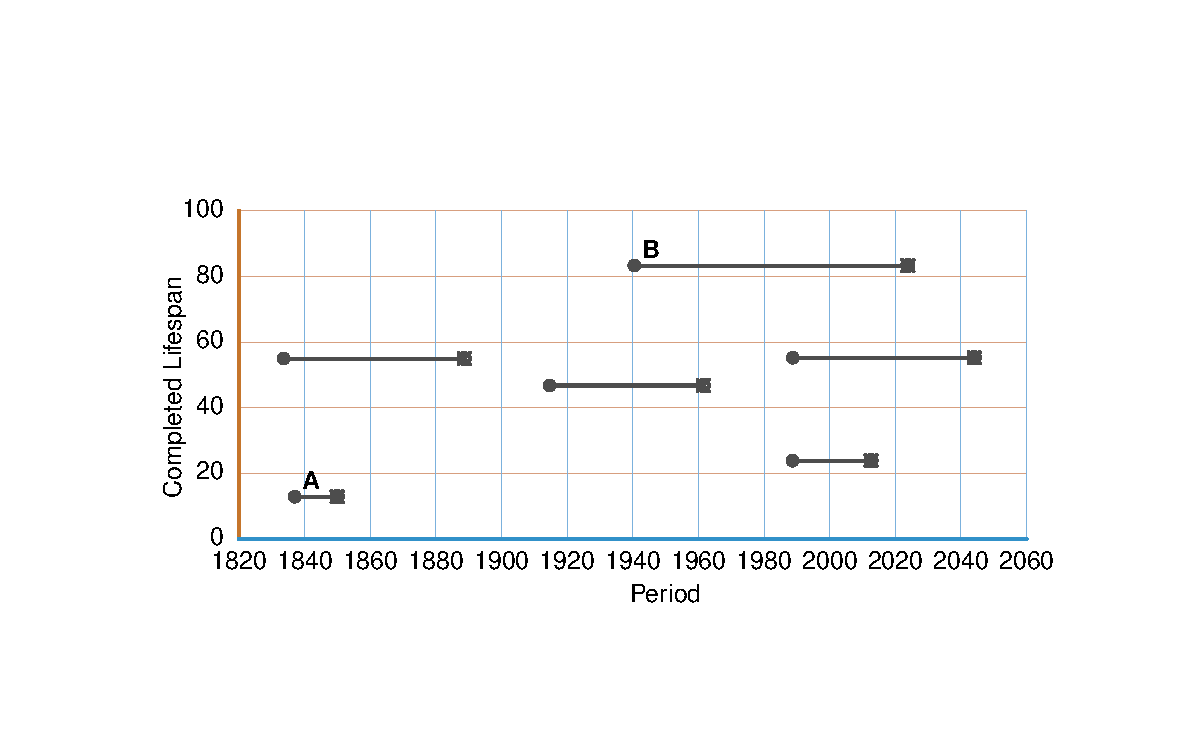
\includegraphics[scale=.7]{Figures/LPdiagram.pdf}
\caption{LP diagram, with example lifelines. Lifeline \textbf{A} starts with a birth (solid circle) in 1836, and ends with a death (crossed circle) in 1849. Lifeline \textbf{B} starts with a birth in 1940, and ends with a death in 2023. The ordinate position L is equal to the length of each life.}
\label{fig:lpd}
\end{figure}

Fig.~\ref{fig:lpq} displays the Qu\'{e}bec population structure on an LP surface. Higher $y$ values correspond to longer lives, and therefore more overlapped underlying lifelines. The upper regions of the surface are thus smoother with respect to time than lower regions. Growth over time in to-be-long-lived individuals could occur due to population growth or mortality improvement. We know this pattern is not due to migration because this population was mostly closed in this time. For Qu\'{e}bec, increasing contours over time are primarily due to population growth. 

Shorter lives (lower L) reveal the rhythms of mortality, adding a peculiar relief to the surface. High-mortality years are marked with vertical cliffs in population structure: Right-aligned cliffs are found on the LP surface when many lives over a range of ages are simultaneously extinguished. These vertical rifts trace back to births over a range of years, producing the -45$\circ$ feature 
\includegraphics{Figures/LP_mort_tri.pdf}. Mortality shocks therefore produce raised triangle relief pattern in population structure. A single isolated year with an extremely high number of births could produce a raised left-edge, but fertility shocks of this kind are far less prominent than mortality shocks in this population. Some known epidemics are marked below the surface with red strips \citep[cf Figure 1.1][]{mazan2011} 

\begin{figure}
\centering
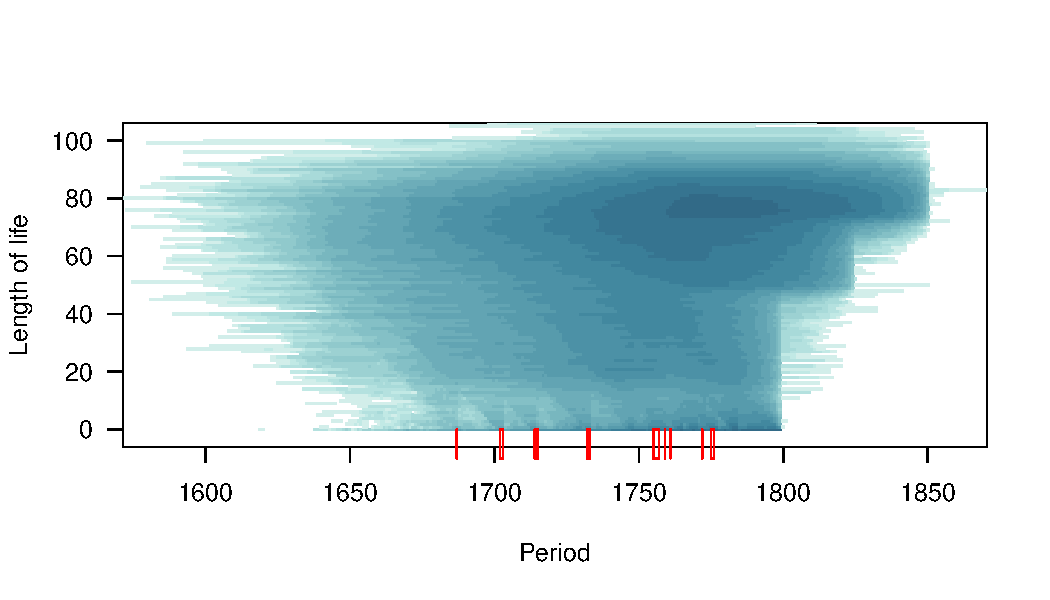
\includegraphics[scale=.9]{Figures/QuebecLP.pdf}
\caption{Population structure by length of life and year. Logged counts}
\label{fig:lpq}
\end{figure}

The inverted step pattern on the right edge of this surface betrays some of the peculiarities of data collection for this source. Death information comes from burial records, which had some age constraints in data collection, depending on the period: For occurrence years 1800 to 1825 only deaths in ages 50 and greater were collected. For the years 1826 to 1850, only deaths in ages 75 and greater were collected. Exceptions to this block edge structure owe to the use of multiple potential sources for death dates. Since lifelines accrue to the LP surface only after deaths occur, the right-side region of Fig.~\ref{fig:lpq} is in a sense incomplete: further increments will happen as death data are added to the series. This kind of structural missingness is less the case for shorter lives, which accrue quickly to the surface due to their very shortness.

\FloatBarrier
\subsection*{TC: Time-to-death and Cohort}

The time-to-death T distribution of a closed birth cohort C reveals its life table. Fig.~\ref{fig:tcd} shows an example TC diagram, where C is in abscissa and T is the ordinate variable. A lifeline on the CT plane is drawn as a vertical segment extending downward from birth until death on the bottom axis. For example, lifeline \texbf{A} represents an individual born in 1624 and dying at age 20 in 1644. In an aggregate of population exposure, this lifeline contributes 1 to the count in each time step descending from 20 to 0 --- the entire countdown timeline. Since each member of a birth cohort eventually comes to die, the coordinate $T = 0$ is maximally heterogeneous with respect to any of the other demographic time measures (A,L,P,D), and lifeline overlap decreases in higher T.

\begin{figure}
\centering
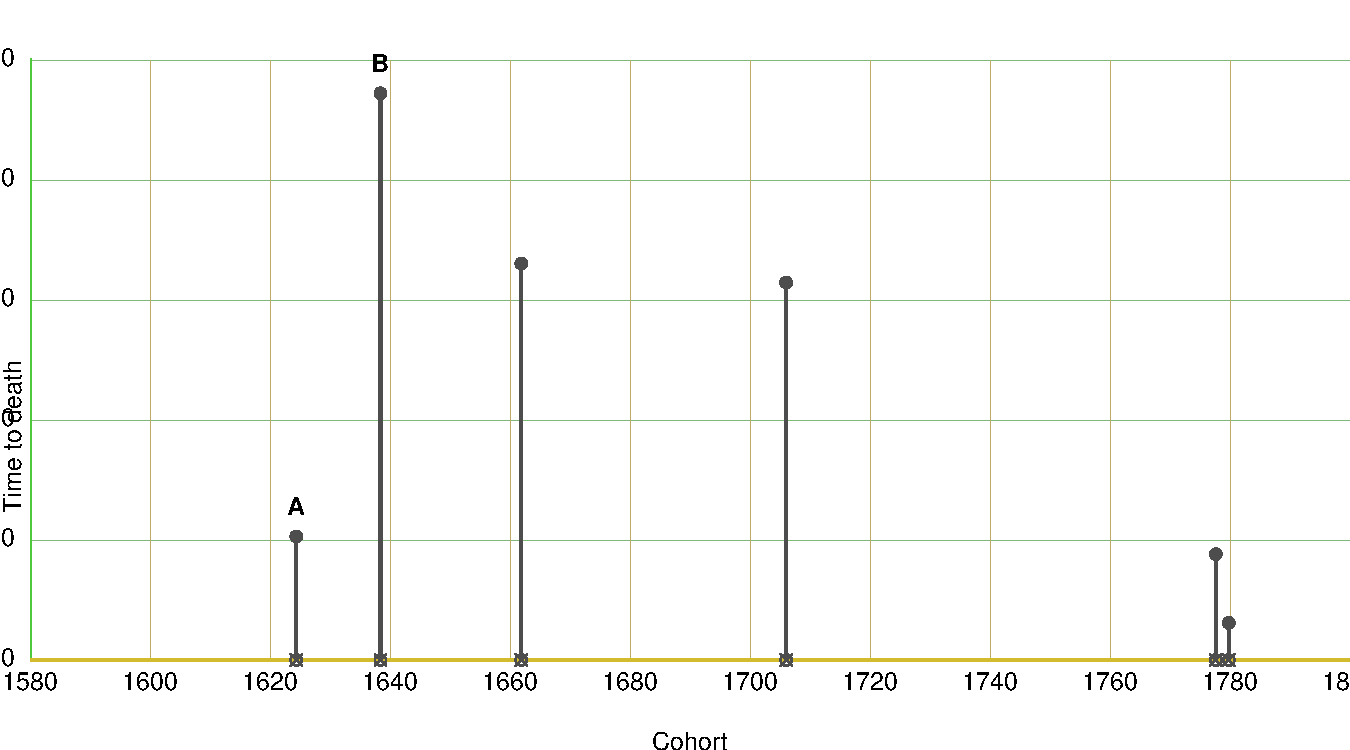
\includegraphics[scale=.6]{Figures/TCdiagram.pdf}
\caption{TC diagram, with example lifelines. Lifeline \textbf{A} is from the 1624 birth cohort, and starts with a birth (solid circle) with 20 remaining years of life, and ends with a death (crossed circle) on the bottom axis (year 1644). Lifeline \textbf{B} is from the 1638 birth cohort, starting with 94 remaining years of life at birth, and ending with death in 1732.}
\label{fig:tcd}
\end{figure}

Fig.~\ref{fig:tcq} shows a TC tabulation of the Quebec population structure. A few features of this surface stand out to the eye. First, as a cohort ages, vertical strips are completed upwards. Ergo, the lower regions of the surface are essentially complete, and the slanted step structure on the right edge of the surface corresponds to the block-step pattern of the LP surface in Fig~\ref{fig:lpq}. Second, the relatively sparse earlier cohorts are visible as vertical strips. This pattern is due to left-censoring on the moment of migration. As the series progresses rightward the cohort experience becomes completely described in the closed population renewal, making the series smoother. In general, we see the population grow as birth year advances. If one were to normalize cohort size to something constant then the surface would closely resemble an AC Lexis surface of survivorship.

\begin{figure}
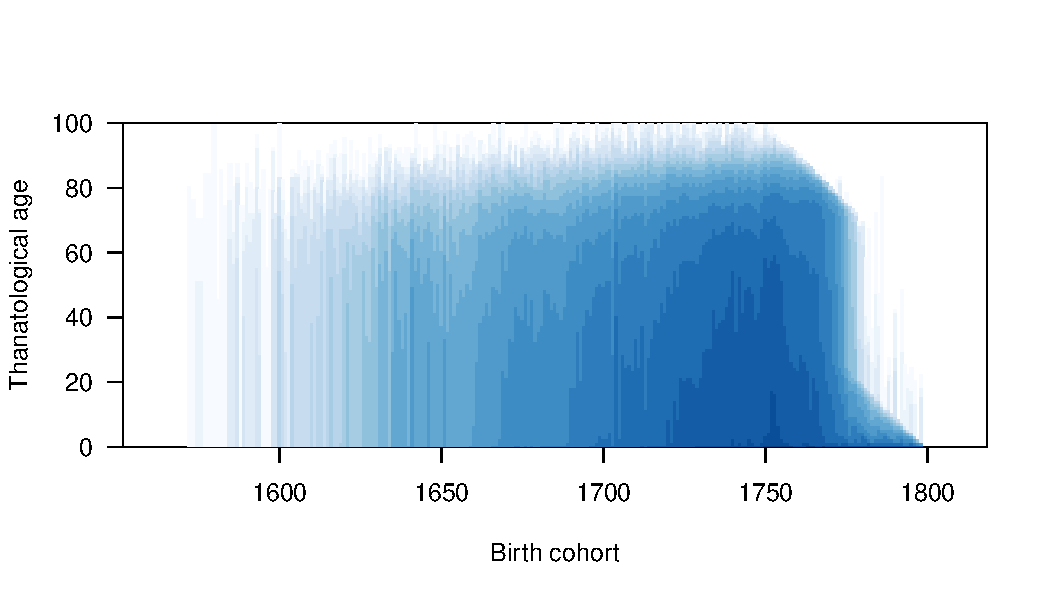
\includegraphics[scale=.9]{Figures/QuebecTC.pdf}
\caption{Population structure by time to death and birth cohort.}
\label{fig:tcq}
\end{figure}

\FloatBarrier
\subsection*{AD}

\begin{figure}
\centering
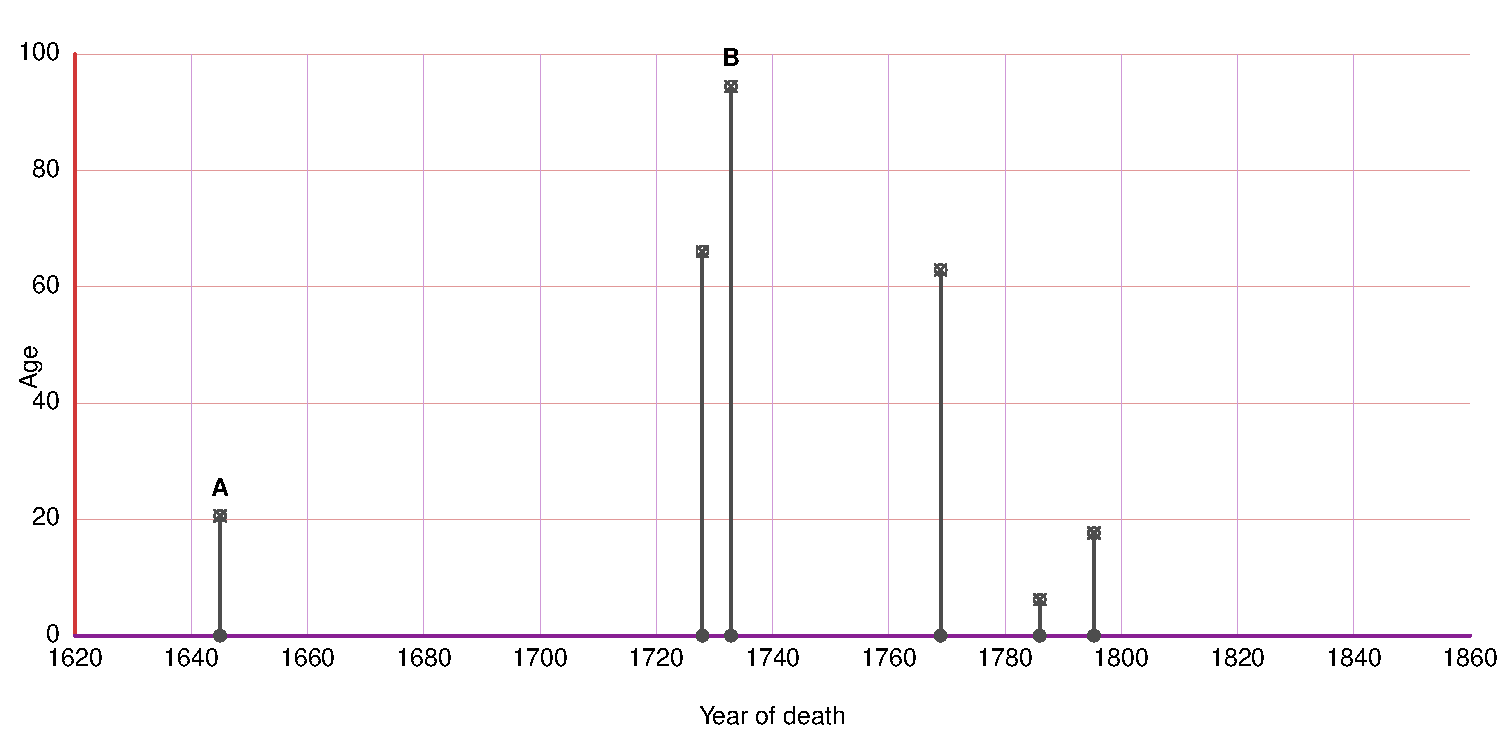
\includegraphics[scale=.6]{Figures/ADdiagram.pdf}
\caption{AD diagram, with example lifelines (same as in previous diagrams). Lifeline \textbf{A} is destined to die in 1644, starting with a birth (solid circle) at age 0, and ending with a death (crossed circle) on at age 20. Lifeline \textbf{B} is destine to die in 1732, starting at age 0 and rising to a death at age 94 in 1732.}
\label{fig:tcd}
\end{figure}
For a given age A, the distribution of the death cohort D of individuals gives the conditional life table, conditional on reaching the given age A, and hence gives, for example, the remaining life expectancy and the variability of remaining life, among other summaries of the
conditional life table. Conversely, for a given death cohort D, the distribution of age A of individuals specifies the distribution of their birth cohorts and life lengths.

\begin{figure}
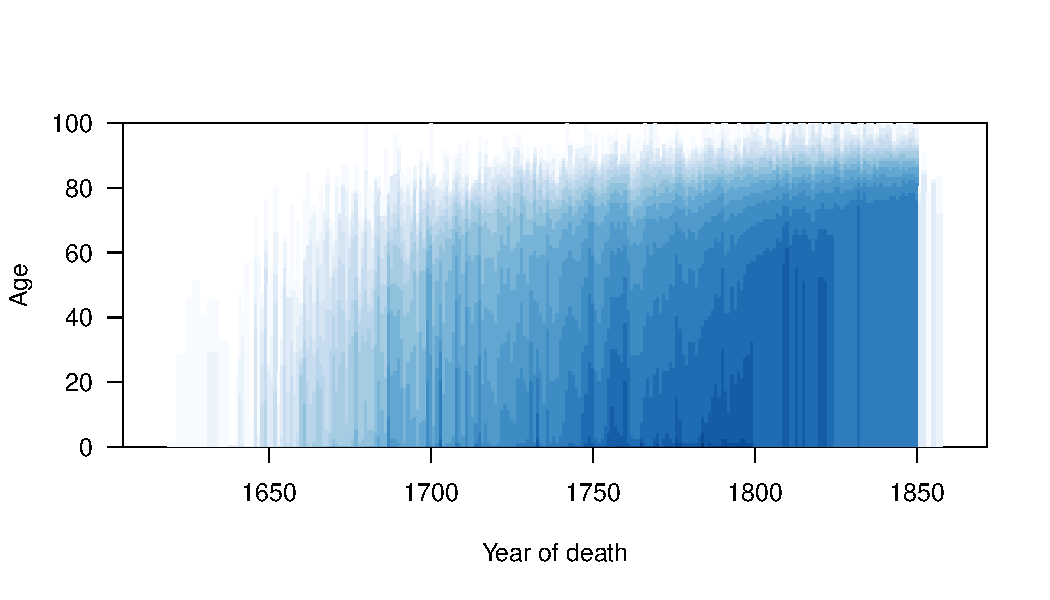
\includegraphics[scale=.9]{Figures/QuebecAD.pdf}
\caption{Population structure by age and year of death.}
\label{fig:adq}
\end{figure}
In the AD plane, we have the same sort of vertical overlap. Just as everyone experiences T = 0, everyone is also included in A = 0 here. If this were a stationary population then a vertical strip here would be equal to one from the CT plane, but we have lots of non-stationary things happening. Vertical striation here is due to mortality shocks in particular years, and these are strictly positive. Anything dearthy-looking is either due to a 'harvest' or data collection oddities. At least I've never heard of a survival shock. So, to repeat, an individual born in 1700 destined to die at age 80 is located at 1780 in the x axes, and ages from the bottom up. Ergo, the bottom of the surface is young people, as we're used to, but they come from different birth cohorts. As with CT, the population is maximally mixed with respect to C (or L or P or T) at A = 0. An 80 year old and an infant dying in 1780 both contribute to the count at age 0 in 1780.

We see here the same high density in death year 1705 that we detected in the LP plane, so maybe it is not a data artifact. Whether there are also high densities of deaths in the other years we identified in the LP plane is not so clear to me; perhaps yes. There appear to be little white rectangles between 1760 and 1800 at ages zero through perhaps 3 or 4. Every lifeline must extend to age zero, so something is wrong here, I think. Again we see the upper envelope increasing with the year of death and rising contour lines.

\FloatBarrier
\section*{Independent time surfaces as cross-sections}
Here use example of HRS prevalence surfaces produced at novel \emph{cut} angles. I'm thinking maybe small multiples, since each would be a fly-through of cross sections in fixed intervals. There would be 3 independent fly-throughs, and 4 Lexis-like fly throughs. These would be  like Fig.~(7) of \cite{riffe2017demographictime}, which is a fly-though at the TAL viewing angle. So, maybe each fly-through is a column and each perspective is a row? Maybe 10-year jumps in columns to imply 3-4 columns? Total? For example, each TAL slice in that Fig 7 is held for a fixed C. It would have been possible to hold P or D fixed instead, but I guess the actually slices would be identical, just the labels would change. Just need to be clear about it when labelling said panel figure.


%%%%%%%%%%%%%%%%%%%%%%%%%%%%%%%%%%%%%%%%%%%%%%
%%                                          %%
%% Backmatter begins here                   %%
%%                                          %%
%%%%%%%%%%%%%%%%%%%%%%%%%%%%%%%%%%%%%%%%%%%%%%

\begin{backmatter}

\section*{Funding}
  \censor{TR} thanks the \censor{Max-Planck-Institute for Demographic Research} for supporting this work with a fair salary. 
  
\section*{Competing interests}
  The authors declare that they have no competing interests.

\section*{Author's contributions}
  Both authors conceived of this project, undertook formal analysis, validation, drafting, and reviewing of the manuscript. \censor{TR} did the data analysis, coding, visualization, and reproducibility repository curation.

\section*{Acknowledgements}
  We wish to thank N reviewers in advance for sharing their time and expertise in reviewing this manuscript. We are also thankful for comments and advice from \censor{Maarten Bijlsma}, \censor{Jonas Sch\"oley}, \censor{Alyson van Raalte}, and \censor{Francisco Villavicencio}.
%%%%%%%%%%%%%%%%%%%%%%%%%%%%%%%%%%%%%%%%%%%%%%%%%%%%%%%%%%%%%
%%                  The Bibliography                       %%
%%                                                         %%
%%  Bmc_mathpys.bst  will be used to                       %%
%%  create a .BBL file for submission.                     %%
%%  After submission of the .TEX file,                     %%
%%  you will be prompted to submit your .BBL file.         %%
%%                                                         %%
%%                                                         %%
%%  Note that the displayed Bibliography will not          %%
%%  necessarily be rendered by Latex exactly as specified  %%
%%  in the online Instructions for Authors.                %%
%%                                                         %%
%%%%%%%%%%%%%%%%%%%%%%%%%%%%%%%%%%%%%%%%%%%%%%%%%%%%%%%%%%%%%

% if your bibliography is in bibtex format, use those commands:
\bibliographystyle{spbasic} % Style BST file (bmc-mathphys, vancouver, spbasic).
\bibliography{references.bib}      % Bibliography file (usually '*.bib' )
% for author-year bibliography (bmc-mathphys or spbasic)
% a) write to bib file (bmc-mathphys only)
% @settings{label, options="nameyear"}
% b) uncomment next line
%\nocite{label}

% or include bibliography directly:
% \begin{thebibliography}
% \bibitem{b1}
% \end{thebibliography}

%%%%%%%%%%%%%%%%%%%%%%%%%%%%%%%%%%%
%%                               %%
%% Figures                       %%
%%                               %%
%% NB: this is for captions and  %%
%% Titles. All graphics must be  %%
%% submitted separately and NOT  %%
%% included in the Tex document  %%
%%                               %%
%%%%%%%%%%%%%%%%%%%%%%%%%%%%%%%%%%%

%%
%% Do not use \listoffigures as most will included as separate files

%\section*{Figures}
%  \begin{figure}[h!]
%  \caption{\csentence{Sample figure title.}
%      A short description of the figure content
%      should go here.}
%      \end{figure}

%\begin{figure}[h!]
%  \caption{\csentence{Sample figure title.}
%      Figure legend text.}
%      \end{figure}

%%%%%%%%%%%%%%%%%%%%%%%%%%%%%%%%%%%
%%                               %%
%% Tables                        %%
%%                               %%
%%%%%%%%%%%%%%%%%%%%%%%%%%%%%%%%%%%

%% Use of \listoftables is discouraged.
%%
%\section*{Tables}
%\begin{table}[h!]
%\caption{Sample table title. This is where the description of the table should go.}
%      \begin{tabular}{cccc}
%        \hline
%           & B1  &B2   & B3\\ \hline
%        A1 & 0.1 & 0.2 & 0.3\\
%        A2 & ... & ..  & .\\
%        A3 & ..  & .   & .\\ \hline
%      \end{tabular}
%\end{table}

%%%%%%%%%%%%%%%%%%%%%%%%%%%%%%%%%%%
%%                               %%
%% Additional Files              %%
%%                               %%
%%%%%%%%%%%%%%%%%%%%%%%%%%%%%%%%%%%

%\section*{Additional Files}
%  \subsection*{Additional file 1 --- Sample additional file title}
%    Additional file descriptions text (including details of how to
%    view the file, if it is in a non-standard format or the file extension).  This might
%    refer to a multi-page table or a figure.

%  \subsection*{Additional file 2 --- Sample additional file title}
%    Additional file descriptions text.


\end{backmatter}
\end{document}
